%\documentclass[a4paper,twoside,10pt,openright]{report}%Dokumentenklasse 
\usepackage{graphicx} %Compiler

\usepackage{dsfont}

%%%% Schrift und Kodierung %%%%
	\usepackage[T1]{fontenc} %Zeichensatzkodierung von 7bit auf 8bit 
	\usepackage[utf8]{inputenc} %Zeichensatzkodierung Unicode bzw. UTF8
	\usepackage{lmodern} %Vektorschrift
	%\RequirePackage[english,spanish,es-nolayout]{babel}
	\usepackage[english]{babel}
	\usepackage{textcomp}
	\usepackage{lmodern}
	\usepackage{url}
	\usepackage[bookmarksnumbered=true]{hyperref}
    \graphicspath{{figures/}}	
	
%%% COLORS %%%
\newcommand{\hl}[1]{
   \textcolor{MidnightBlue!90!black}{#1} 
}

\usepackage{pifont}% http://ctan.org/pkg/pifont
\newcommand{\cmark}{\ding{51}}%
\newcommand{\xmark}{\ding{55}}%

\usepackage{stackrel}

\usepackage{feynmp}

\usepackage{amsthm}
\newtheorem{definition}{Definition}
\newtheorem{proposition}{Proposition}
	
%%%% Fancy Header %%%
\usepackage{fancyhdr}
\usepackage[dvipsnames]{xcolor}
\usepackage{tikz} 
\usepackage{pgfplots}
%\usepackage{pgf-pie}

\usetikzlibrary{arrows}
\usetikzlibrary{shapes.geometric, arrows}

\definecolor{mycolor}{rgb}{0.45,0.45,0.45}% dark grey

\newcommand{\mcD}{\mathcal{D}}
\newcommand{\mcL}{\mathcal{L}}
\newcommand{\dth}{\Delta_{\text{th/sys}}}
\newcommand{\dst}{\Delta_{\text{stat}}}
\newcommand{\dsy}{\Delta_{\text{syst}}}
\newcommand{\sthsy}{\sigma_{\text{th/sys}}}
\newcommand{\sth}{\sigma_{\text{th}}}
\newcommand{\sst}{\sigma_{\text{stat}}}
\newcommand{\ssy}{\sigma_{\text{syst}}}

\newcommand{\Langle}{\big\langle}
\newcommand{\Rangle}{\big\rangle} 
 
\fancyhf{}
\fancyhead[LE]{\sffamily\color{mycolor}\nouppercase{\leftmark}} % left even, right odd
\fancyhead[RO]{\sffamily\color{mycolor}\nouppercase{\rightmark}} % left even, right odd
\fancyfoot[CE,CO]{\sffamily\color{mycolor}\nouppercase{\thepage}} % center even, center odd
\renewcommand{\headrule}{{\color{mycolor}%
\hrule width\headwidth height\headrulewidth \vskip-\headrulewidth}}
\renewcommand{\headrulewidth}{0.5pt}

\fancypagestyle{plain}{%
    \fancyhf{}%
    \fancyfoot[CE,CO]{ { \sffamily\color{mycolor}{\thepage} } }
	\renewcommand{\headrulewidth}{0.0pt}
}

%\fancypagestyle{fancy}{%
%   \fancyhf{}
%	\fancyhead[LE,RO]{\sffamily\color{mycolor}\nouppercase{\leftmark}} % left even, right odd
%	\fancyfoot[CE,CO]{\sffamily\color{mycolor}\nouppercase{\thepage}} % center even, center odd
%	\renewcommand{\headrule}{{\color{mycolor}%
%	\hrule width\headwidth height\headrulewidth \vskip-\headrulewidth}}
%	\renewcommand{\headrulewidth}{0.5pt}
%}


%%% Customize titles %%%%
\usepackage[ ]{titlesec}  %
\usepackage{etoolbox}
\makeatletter
\patchcmd{\ttlh@hang}{\parindent\z@}{\parindent\z@\leavevmode}{}{}
\patchcmd{\ttlh@hang}{\noindent}{}{}{}
\makeatother
%\titleformat{\chapter}[display]
%  { \normalsize \huge  \color{black}}%
%  {\flushright \normalsize \color{mycolor} \MakeUppercase %
%  {\sffamily \chaptertitlename } \hspace{1 ex}%
%  { \fontsize{60}{60}\selectfont \color{mycolor} \sffamily  \thechapter }}%
%  {10 pt}%
%  {\sffamily \huge \color{mycolor}\bfseries}
%\newcommand\mychapformat[1]{\parbox[t]{\dimexpr\textwidth-3em\relax}{\raggedleft#1}}
\titleformat{\chapter}[hang]{\Huge\bfseries\color{mycolor}\sffamily}% the number
	{\thechapter\hspace{20pt}\textcolor{mycolor}{|}\hspace{20pt}}%
	{0pt}{\Huge\bfseries\color{mycolor}\sffamily}% the title
\titleformat*{\section}{\sffamily\LARGE\color{mycolor}}
\titleformat*{\subsection}{\sffamily\Large\color{mycolor}}
\titleformat*{\subsubsection}{\sffamily\large\color{mycolor}}
\titleformat*{\paragraph}{\sffamily\large\bfseries\color{mycolor}}



	
%%%% Mathepakete %%%%
	\usepackage{array}
	\usepackage{calc}
	\usepackage{amsmath}
	\usepackage[intlimits]{empheq}
	\usepackage{amssymb,mathrsfs}
	\usepackage{theorem}
	\usepackage{slashed}
	\usepackage{feynmp-auto}

%%%% Sonstiges %%%%
	%\usepackage{subcaption}
	\expandafter\def\csname ver@subfig.sty\endcsname{}
	\usepackage{subfig} %Ermöglicht subfloats, also mehrere Tabellen/Bilder in einer Umgebung
	\usepackage{float} %Setzt mit [H] Figuren genau dort hin, wo sie im Text auftauchen
	\usepackage{booktabs} %Andere Tabellen
	\usepackage{gensymb}
	\usepackage{extarrows}%lange Pfeile
%	\usepackage{pst-pdf}	
	\usepackage{wasysym} %Symbolpaket
	\usepackage{multirow} %Ein Wert für mehrere Zeilen oder Spalten von Tabellen. Verwendung \multirow{#AnzahlZeilen}{*}{Name} bzw. analog \multicolumn{}{}{}
	\usepackage{rotating} %ermöglicht Schiefe Schrift
	%\usepackage{ziffer} %Deutsche Zahlen (Komma als Dezimalstelle im Mathemodus!)
	\usepackage{nicefrac} %Im Text schöne Brüche
	\usepackage[inner=3cm, outer=2.4cm, top=3cm]{geometry} %Passt Seitenränder an (left, right, top, bottom, width, height, textwidth, textheight)
	\usepackage{scrhack} %Verbessert angeblich LaTeX-Pakete
	\usepackage{numprint} %ROOT-Zahlen in deutsches zahlenformat übertragen. Syntax: \numprint[kg]{1.234e56} wird zu 1,234 * 10^56 kg
	\usepackage{cite}
	\usepackage{placeins}
	\usepackage{changepage}
	%\hyphenation{con-fine-ment}
	
%%%% spezielle Formatierungen %%%%
	\setlength{\emergencystretch}{25pt} %verhindert das Herausragen von Wörtern übers Zeilenende
	\setlength{\parindent}{0pt} %Kein Einschub bei neuem Absatz
	\setlength{\parskip}{2pt plus 1pt} %Erhöht Abstand zwischen Absätzen (um 1pt flexibel bei Seitenumbrüchen)
	
	%%%% Dokument-Variablen %%%%
\date{\today}

%%%% Eigene Befehle %%%%
\DeclareGraphicsRule{*}{mps}{*}{}
	\newcommand{\mE}[1]{\,\mathrm{#1}} %Einheiten im Mathemodus
	\renewcommand{\sl}[1]{\slashed{#1}} %Feynman-Slash
	\newcommand{\dummyImage}[2]{  %Erzeugt eine Umgebung wie includegraphics
		\frame{\mbox{\rule{0pt}{#2}	Bild fehlt  noch \rule{#1}{0pt}}}
	}
	\renewcommand{\i}{\mathrm{i}} %Imaginäre Einheit
%	\renewcommand{\vec}[1]{\textbf{#1}} %Fette Vektoren
	\newcommand{\bc}{\begin{center}}
	\newcommand{\ec}{\end{center}}

\newcommand{\matM}{\mathcal{M}}
\newcommand{\matH}{\mathcal{H}}
\newcommand{\matS}{\mathcal{S}}
\newcommand{\matU}{\mathcal{U}}
\newcommand{\matUL}{\mathcal{U}_L}
\newcommand{\matUR}{\mathcal{U}_R}

%%% center all the figures and tables
\makeatletter
\g@addto@macro\@floatboxreset\centering
\makeatother

%% maximal number of floating environments on each page 
\setlength{\floatsep}{0pt}
\setcounter{topnumber}{1}
\setcounter{bottomnumber}{1}
\setcounter{totalnumber}{1}
\renewcommand{\topfraction}{1.0}
\renewcommand{\bottomfraction}{1.0}
\renewcommand{\textfraction}{0.0}
\renewcommand{\thefootnote}{\fnsymbol{footnote}}

\def\tablename{Table}
\def\figurename{Figure}

\newcommand{\newparagraph}{\par\bigskip\noindent}
\newcommand{\toolfont}[1]{\texttt{#1}}
\newcommand{\ord}{\ensuremath{\mathcal{O}}}
\newcommand{\ope}[1]{\ensuremath{\mathcal{O}_{#1}}}
\newcommand{\largex}{\ensuremath{\large \boldsymbol{\times}}}
\newcommand{\brlargex}{\ensuremath{\large (\boldsymbol{\times})}}
\newcommand{\mheavy}{\ensuremath{M}}

\newcommand{\lag}{\ensuremath{\mathcal{L}}}
\newcommand{\mat}{\ensuremath{\mathcal{M}}}
\newcommand{\delx}{\ensuremath{\Delta}}
\newcommand{\data}{\ensuremath{\mathcal{D}}}
\newcommand{\jump}{\vspace{0.3cm}}
\newcommand{\bsg}{\ensuremath{\mathcal{B}(b \to s \gamma)}}
\newcommand{\rself}{\ensuremath{\hat{\Sigma}}}
\newcommand{\retildehat}{\ensuremath{\mbox{Re}\hat{\Sigma}}}
\newcommand{\retilde}{\ensuremath{\mbox{Re}\,\Sigma}}
\newcommand{\dweaksing}{\ensuremath{\delta_{\text{weak}}^{\text{sing}}}}
\newcommand{\dweak}{\ensuremath{\delta_{\text{weak}}}}
\newcommand{\newtext}[1]{\textcolor{red}{#1}}
\newcommand{\suit}{\textcolor{blue}{$\spadesuit$}}
\newcommand{\neutn}{\ensuremath{\tilde{\chi}^0_n}}
\newcommand{\gluino}{\ensuremath{\tilde{g}}}
\newcommand{\squark}{\ensuremath{\tilde{q}}}
\newcommand{\met}{\ensuremath{\slashed{E}_T}}
\newcommand{\nqsq}{\ensuremath{\tilde{\chi}\,\tilde{q}\,q}}
\newcommand{\msbar}{\ensuremath{\overline{MS}}}
\newcommand{\sw}{\ensuremath{s_w}}
\newcommand{\swd}{\ensuremath{s^2_w}}
\newcommand{\cw}{\ensuremath{c_w}}
\newcommand{\cwd}{\ensuremath{c^2_w}}
\newcommand{\myrbox}[1]{\parbox{4.0cm}{#1}}

\usepackage{xspace}
\newcommand{\brinv}{\ensuremath{BR_{\text{inv}}}\xspace}
\newcommand{\vegas}{\textsc{Vegas}\xspace}
\newcommand{\madgraph}{\textsc{Madgraph}\xspace}
\newcommand{\geant}{\textsc{Geant4}\xspace}
\newcommand{\pythia}{\textsc{Pythia}8\xspace}
\newcommand{\fastjet}{\textsc{FastJet}\xspace}
\newcommand{\delphes}{\textsc{Delphes}\xspace}
\newcommand{\sherpa}{\textsc{Sherpa}\xspace}
\newcommand{\sklearn}{\textsc{scikit-learn}\xspace}
\newcommand{\keras}{\textsc{Keras}\xspace}
\newcommand{\tensorflow}{\textsc{TensorFlow}\xspace}
\newcommand{\pytorch}{\textsc{PyTorch}\xspace}
\newcommand{\theano}{\textsc{Theano}\xspace}
\newcommand{\adam}{\textsc{Adam}\xspace}

\newcommand{\psib}{\overline{\psi}}
\newcommand{\bpm}{\begin{pmatrix}}
\newcommand{\epm}{\end{pmatrix}}

\newcommand{\p}{\partial}
\newcommand{\br}{\text{BR}}
\newcommand{\qqquad}{\qquad \qquad}
\newcommand{\qqqquad}{\qquad \qquad \qquad}

\newcommand{\matx}{|\mathcal{M}|^2}
\newcommand{\really}{\stackrel{!}{=}}
\newcommand{\SFitter}{\textsc{SFitter} }

% units of measure
\newcommand{\mev}{{\ensuremath\rm MeV}}
\newcommand{\gev}{{\ensuremath\rm GeV}}
\newcommand{\tev}{{\ensuremath\rm TeV}}
\newcommand{\fb}{{\ensuremath\rm fb}}
\newcommand{\ab}{{\ensuremath\rm ab}}
\newcommand{\pb}{{\ensuremath\rm pb}}
\newcommand{\sign}{{\ensuremath\rm sign}}
\newcommand{\iab}{\text{ab}^{-1}}
\newcommand{\ifb}{{\ensuremath\rm fb^{-1}}}
\newcommand{\ipb}{{\ensuremath\rm pb^{-1}}}

% really great macro by Chris Lester
\def\slashchar#1{\setbox0=\hbox{$#1$}           % set a box for #1
   \dimen0=\wd0                                 % and get its size
   \setbox1=\hbox{/} \dimen1=\wd1               % get size of /
   \ifdim\dimen0>\dimen1                        % #1 is bigger
      \rlap{\hbox to \dimen0{\hfil/\hfil}}      % so center / in box
      #1                                        % and print #1
   \else                                        % / is bigger
      \rlap{\hbox to \dimen1{\hfil$#1$\hfil}}   % so center #1
      /                                         % and print /
   \fi}
\newcommand{\dslash}{\slashchar{\partial}}
\newcommand{\Dslash}{\slashchar{D}}

\def\eg{{e.g.}\ }
\def\ie{{i.e.}\ }
%\def\etal{{\sl et al} \,}
%\DeclareMathOperator{\tr}{Tr}
\newcommand{\pbp}{\ensuremath{H^\dagger\,H}}
\DeclareMathOperator{\tr}{Tr}
\newcommand{\Dfb}{\mbox{$\raisebox{2mm}{\boldmath ${}^\leftrightarrow$}\hspace{-4mm} D$}}
\newcommand{\Dfba}{\mbox{$\raisebox{2mm}{\boldmath ${}^\leftrightarrow$}\hspace{-4mm} D^a$}}
\newcommand{\overbar}[1]{\mkern 1.5mu\overline{\mkern-1.5mu#1\mkern-1.5mu}\mkern 1.5mu}
\let\vec\mathbf % vectors in bold
\renewcommand{\d}{\text{d}}


%\pagestyle{fancy}
%\graphicspath{{../figures/}}	
%\begin{document}

\chapter{Latent Space Refinement}\label{chap:lsr}
\enlargethispage{2ex}
\vspace*{-2pt}

\enlargethispage{2ex}

\section*{Abstract}
{\bf Deep generative models are becoming widely used across science and industry for a variety of purposes. A common challenge is achieving a precise implicit or explicit representation of the data probability density.  Recent proposals have suggested using classifier weights to refine the learned density of deep generative models.  We extend this idea to all types of generative models and show how latent space refinement via iterated generative modeling can circumvent topological obstructions and improve precision. This methodology also applies to cases were the target model is non-differentiable and has many internal latent dimensions which must be marginalized over before refinement. We demonstrate our Latent Space Refinement (LaSeR) protocol on a variety of examples, focusing on the combinations of Normalizing Flows and Generative Adversarial Networks. We make all codes publicly available.}

\section{Introduction}
\label{sec:intro}

Generative models are essential tools for many aspects of scientific and engineering workflows. First-principles simulations encode physical laws and then samples from these simulations can be used for designing, performing, and interpreting a measurement. However, these physics-based simulations can be too slow or not precise enough for a growing number of studies. Deep learning-based techniques such as Generative Adversarial Networks (GAN)~\cite{Goodfellow:2014:GAN:2969033.2969125,Creswell2018}, Variational Autoencoders (VAE)~\cite{kingma2014autoencoding,Kingma2019}, and Normalizing Flows (NF)~\cite{10.5555/3045118.3045281,Kobyzev2020} are powerful surrogates that can accelerate slow simulations and model complex datasets that would otherwise be intractable to describe from first principles. For example, a growing number of studies are exploring these tools for high energy physics (HEP) applications~\cite{deOliveira:2017pjk,Paganini:2017hrr,Paganini:2017dwg,Alonso-Monsalve:2018aqs,Butter:2019eyo,Martinez:2019jlu,Bellagente:2019uyp,Vallecorsa:2019ked,SHiP:2019gcl,Carrazza:2019cnt,Butter:2019cae,Lin:2019htn,DiSipio:2019imz,Hashemi:2019fkn,Chekalina:2018hxi,ATL-SOFT-PUB-2018-001,Zhou:2018ill,Carminati:2018khv,Vallecorsa:2018zco,Datta:2018mwd,Musella:2018rdi,Erdmann:2018kuh,Deja:2019vcv,Derkach:2019qfk,Erbin:2018csv,Erdmann:2018jxd,Urban:2018tqv,Oliveira:DLPS2017,deOliveira:2017rwa,Farrell:2019fsm,Hooberman:DLPS2017,Belayneh:2019vyx,buhmann2020getting,Alanazi:2020jod,2009.03796,2008.06545,Kansal:2020svm,Maevskiy:2020ank,Lai:2020byl,Choi:2021sku,Rehm:2021zow,Rehm:2021zoz,Carrazza:2021hny,Albergo:2019eim,Kanwar:2003.06413,Brehmer:2020vwc,Bothmann:2020ywa,Gao:2020zvv,Gao:2020vdv,Nachman:2020lpy,Choi:2020bnf,Lu:2020npg,Bieringer:2020tnw,Hollingsworth:2021sii,Monk:2018zsb,Cheng:2020dal,1816035,Howard:2021pos,Buhmann:2021lxj,Bortolato:2021zic,deja2020endtoend,Hariri:2021clz,Fanelli:2019qaq, 1800956, Bellagente:2021yyh}.

A key difference in generative modeling between many scientific applications, including HEP, and typical industrial applications is that individual samples are often not useful. Inference is performed on a statistical basis and so it is essential to model the probability density precisely and not just match its support. Existing deep generative models have shown great promise in qualitatively modeling complex probability densities, but it is often challenging to achieve precision.

A useful strategy to improve the precision of generative models is to refine their predictions. For example, Ref.~\cite{che2020gan} showed how the classification part of a GAN can be used to reweight and resample the input probability distribution of the random noise. A similar idea was introduced in Ref.~\cite{2009.03796} that is not specific to GANs, whereby a classifier network is trained on the generated samples to produce weights that improve the precision of the generated probability distribution. We combine and extent these approaches by introducing the \textbf{La}tent \textbf{S}pac\textbf{e} \textbf{R}efinement (\textsc{LaSeR}) protocol, illustrated in Fig.~\ref{fig:schematic}. Like \textsc{DctrGAN}~\cite{2009.03796,Andreassen:2019nnm}, \textsc{LaSeR} starts with any generative model $g(z)$ and trains a post-hoc classifier to distinguish the generated samples from the target data. A challenge with \textsc{DctrGAN} is that the results are weighted, which reduces the statistical power of a generated sample. The energy-based framework of Discriminator Driven Latent Sampling~(DDLS)~\cite{che2020gan} produces unweighted samples by transferring the weights to the latent space and then performing Langevin Markov Chain Monte Carlo (MCMC) to produce unweighted samples.  

We develop a more general protocol that works for any generative model and is more efficient than the Langevin MCMC approach of Ref.~\cite{che2020gan}. We begin by pulling back the weights from our post-hoc classifier to the latent space, either directly or via the \textsc{OmniFold} method~\cite{Andreassen:2019cjw} when the generator is not surjective. We then propose to learn a second generative model $\Phi(y)$ that maps an auxiliary latent space onto the refined latent space. Generating from the refined model amounts to sampling from the auxiliary latent space and applying $g(\Phi(y))$. We focus on the case where $g$ is a normalizing flow and $\Phi$ is a GAN because GANs need not to be invertible
%\footnote{There are tricks to achieve a similar result for Normalizing Flows~\cite{huang2020augmented}.}
; however, the method can be applied to any pair of generative models. Furthermore, the procedure can be iterated for further refinement.  Learning a post-hoc generative model in a latent space was also studied by the authors of Refs.~\cite{bohm2020probabilistic,pmlr-v37-li15,xiao2019generative}, where a standard autoencoder becomes probabilistic via a second model such as a NF trained on the bottleneck layer. Similarly, the authors of Ref.~\cite{dai2018diagnosing} proposed an iterative VAE setup to bring the latent space closer to a target multidimensional Gaussian random variable.

This paper is organized as follows. We review related work and describe the statistical properties and challenges associated with existing generative models in Section~\ref{sec:background}.  We introduce various ways of implementing the \textsc{LaSeR} protocol in Sec.~\ref{sec:methods}.  Illustrative numerical examples are provided in Sec.~\ref{sec:examples} and the paper ends with conclusions and outlook in Sec.~\ref{sec:conclusion}.

\begin{figure}[h!]
    \centering
    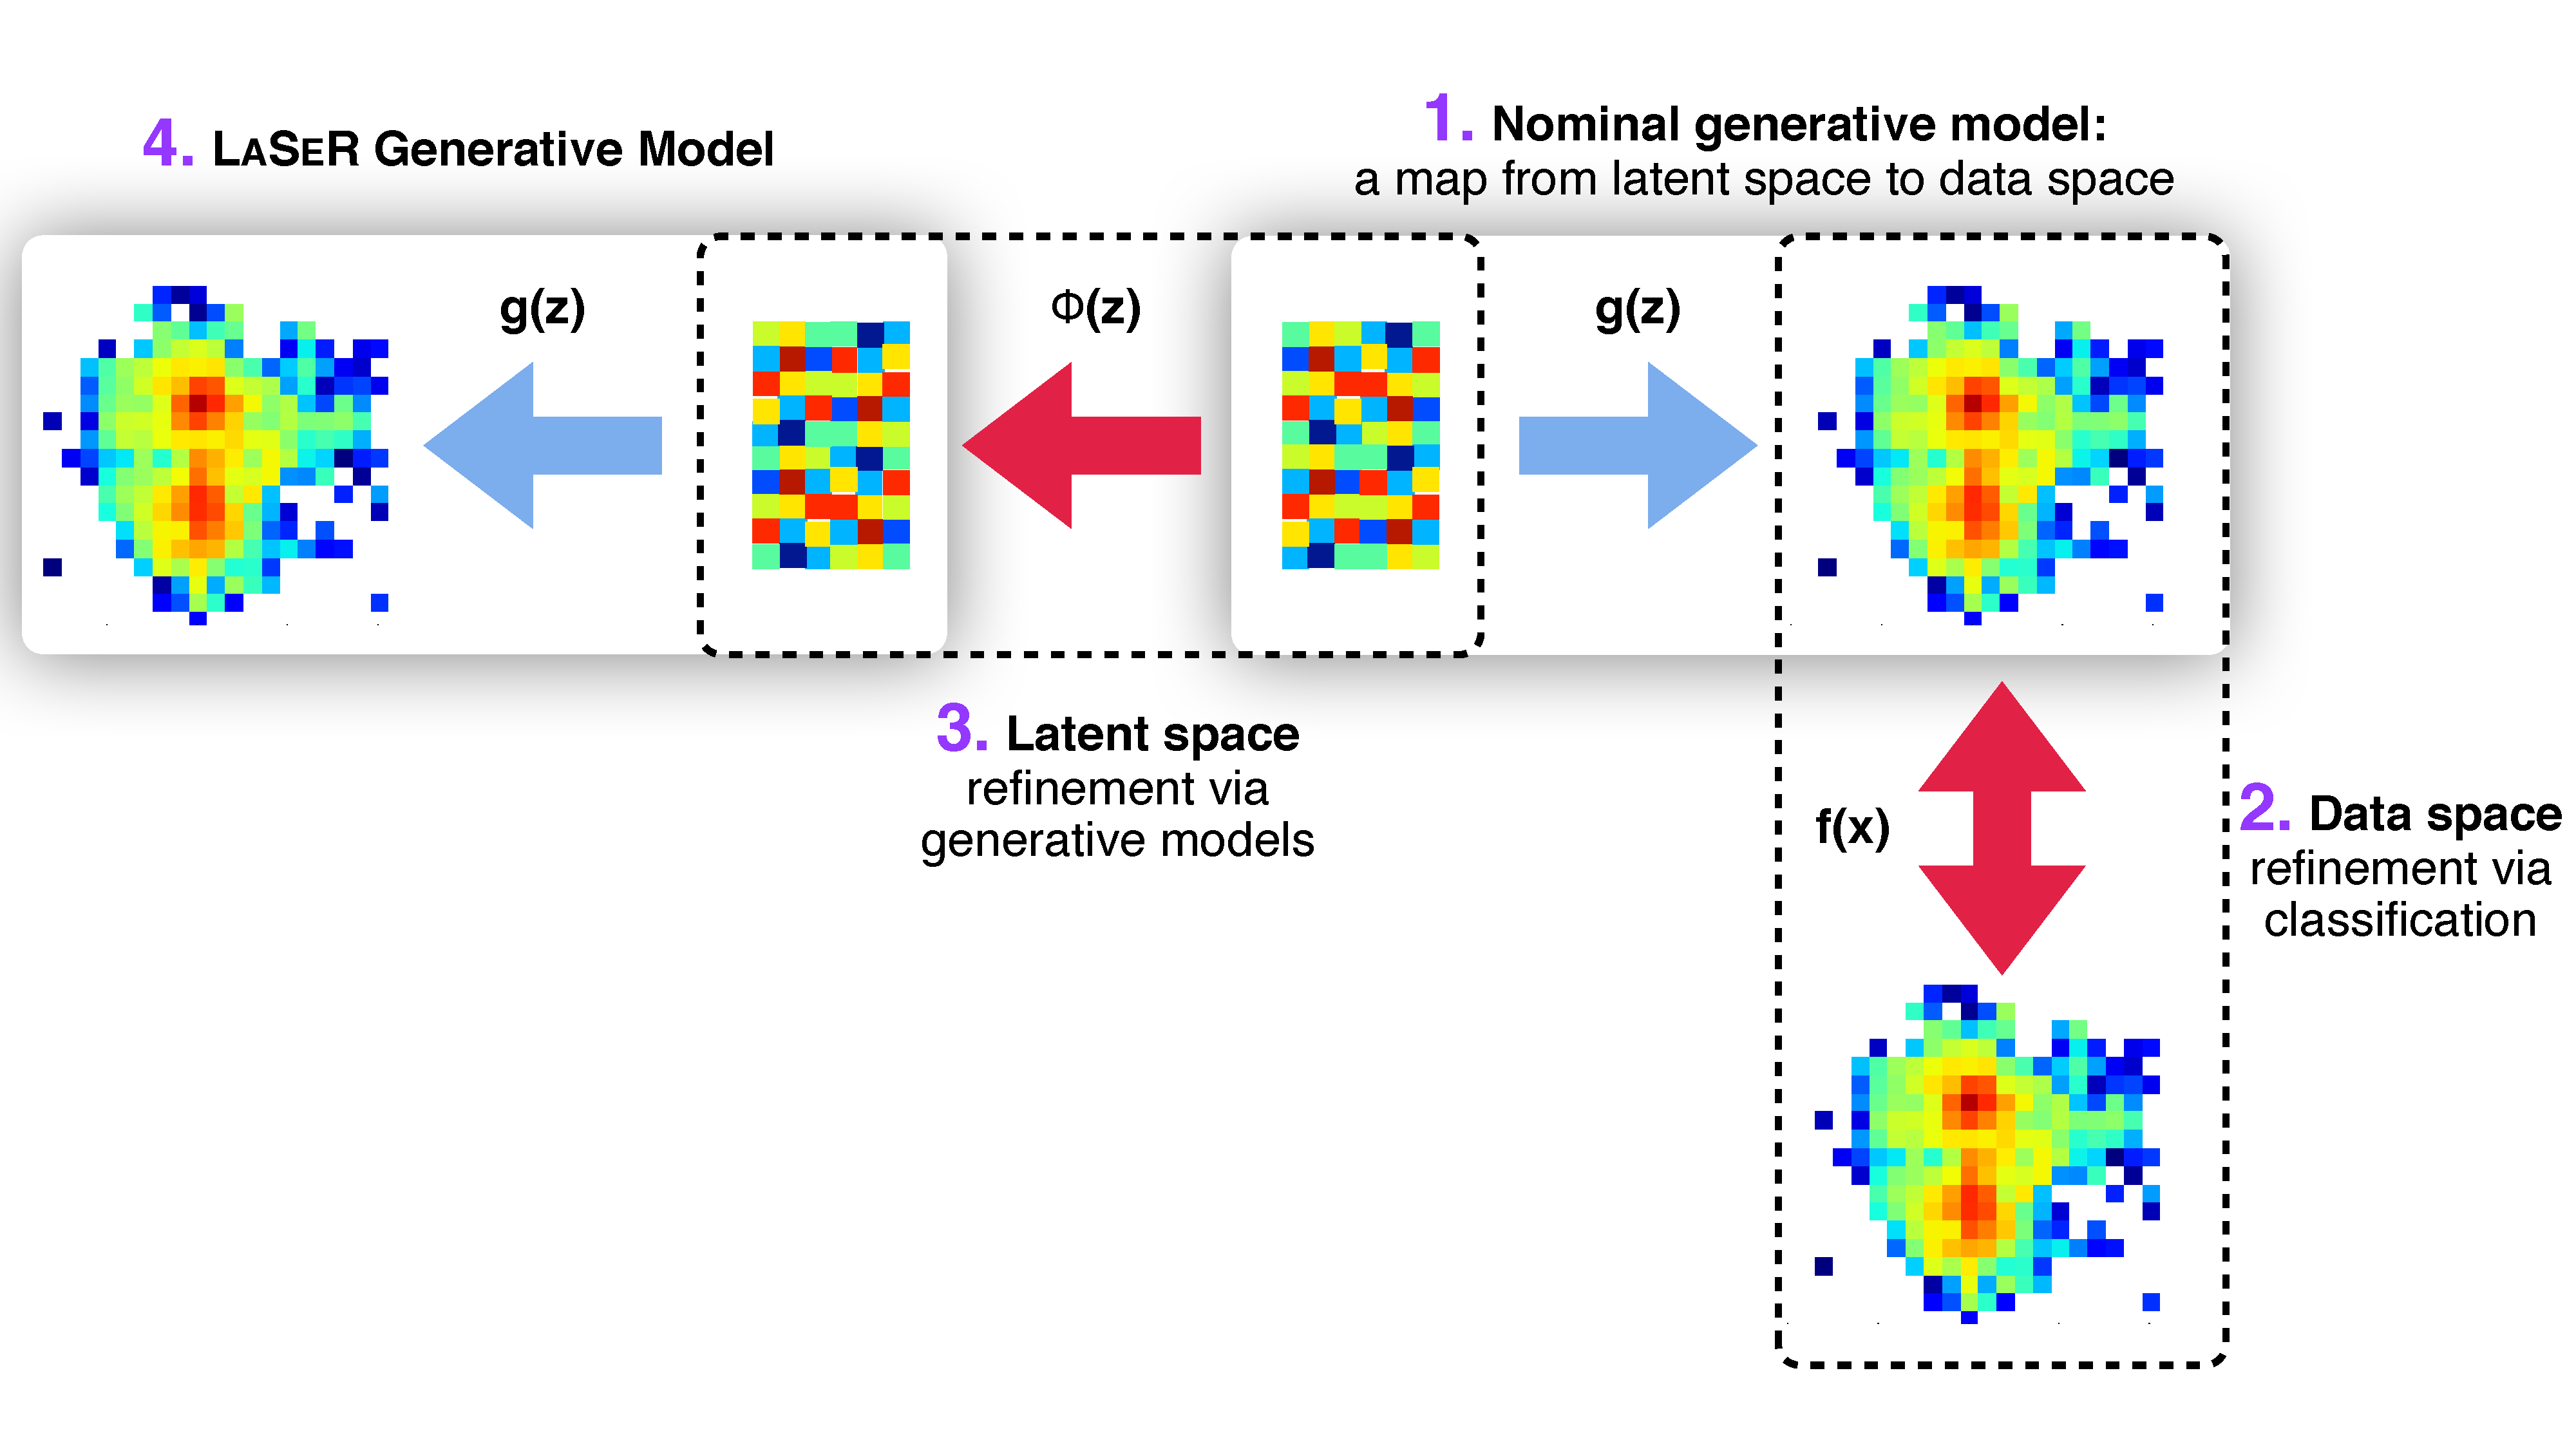
\includegraphics[width=0.95\textwidth]{./figures/LSR/SchematicDiagram.pdf}
    \caption{A schematic diagram illustrating the \textsc{LaSeR} protocol.  {\large\textbf{\color{Fuchsia}1}}. The upper right part of the diagram represents a given generative model $g:\mathbb{R}^N\rightarrow \mathbb{R}^M$ that maps features from a latent space to a data space.  {\large\textbf{\color{Fuchsia}2}}. A classifier network $f:\mathbb{R}^M\rightarrow \mathbb{R}$ is trained to distinguish between the generated samples and real samples from data.  The output of this classifier is interpreted as a likelihood ratio between the generated samples and the real samples and is pulled back to the latent space.  If $f$ is trained with binary cross entropy, the weights are approximated as $w(x)=f(x)/(1-f(x))$ and then the weight of a latent space point $z$ is $w(g(z))$.  {\large\textbf{\color{Fuchsia}3}}. Next, a second generative model $\Phi:\mathbb{R}^L\rightarrow \mathbb{R}^N$ is trained with these weights to transform the original latent space into a new latent space.  {\large\textbf{\color{Fuchsia}4}}. The \textsc{LaSeR} model is then given by $g(\Phi(y))$.}
    \label{fig:schematic}
\end{figure}

%%%%%%%%%%%%%%%%%%%%%%%%%%%%%%%%%%%%%%%
\section{Background}
\label{sec:background}
%%%%%%%%%%%%%%%%%%%%%%%%%%%%%%%%%%%%%%%
A generator is a function $g$ that maps a latent space $\mathcal{Z}\subseteq \mathbb{R}^N$ onto a target or feature space $\mathcal{X}\subseteq \mathbb{R}^M$, with underlying probability densities $p_\mathcal{Z}$ and $p_\mathcal{X}$, respectively.  Typically, $p_\mathcal{Z}$ is chosen to be simple (e.g. normal or uniform) so that it is efficient to generate data $Z\sim p_\mathcal{Z}$.  In some cases, the latent space $\mathcal{Z}$ is broken into two components: one component that specifies the input features of interest and one component that specifies auxiliary latent features that are marginalized over.  When this happens, the map $g$ is viewed as a stochastic function of the first latent space component.  While our examples exclusively cover the case of deterministic maps from the full latent space to the target space, our approach can accommodate both settings as we explain in more detail below.

The function $g$ can be constructed from first-principles insights about the dynamics of a system or it can be learned from data.  For example, commonly-used deep generative models include

\begin{itemize}
    \item Generative adversarial networks (GANs)~\cite{Goodfellow:2014:GAN:2969033.2969125,Creswell2018}
    \item Variational autoencoders (VAEs)~\cite{kingma2014autoencoding,Kingma2019}
    \item Normalizing flows (NFs)~\cite{10.5555/3045118.3045281,Kobyzev2020} %and related  invertible neural networks (INNs)~\cite{ardizzone2019analyzing,1800956}.
    %\item Physics-based Monte-Carlo generators (e.g. from collider physics~\cite{Rambo, Platzer:2013esa, Alwall:2014hca, Sjostrand:2014zea, Frederix:2018nkq,Bellm:2015jjp, Bothmann:2019yzt}).
\end{itemize}

Apart from the specific learning objective, all generative models have their intrinsic advantages and disadvantages. The relevant features to understand the \textsc{LaSeR} protocol are summarized in Table~\ref{tab:comparison} and are further discussed in the following.

%\begin{table}[!htbp]
%  \caption{A comparison of commonly used deep generative models.}
%  \label{tab:comparison}
%  \centering
%  \begin{tabular}{lcccc}
%    \toprule
%      \parbox{3cm}{\centering Method} & \parbox{1.5cm}{\centering Train on data} & \parbox{1.5cm}{\centering Exact log-likelihood} & \parbox{2cm}{\centering  Non-topology preserving} \\ 
%    \midrule
%     Variational Autoencoders & {\color{green!70!black}\cmark} &  {\color{red!80!black}\xmark} & {\color{green!70!black}\cmark}\\
%     Generative Adversarial Networks & {\color{green!70!black}\cmark} & {\color{red!80!black}\xmark} & {\color{green!70!black}\cmark}  \\
%     Normalizing Flows & {\color{green!70!black}\cmark} & {\color{green!70!black}\cmark} & {\color{red!80!black}\xmark}\\
%    \bottomrule
%  \end{tabular}
%\end{table}

%======================================
\subsection{Generative models and coordinate transformations}
\label{sec:event_generation}
%======================================

While the three generative models introduced in the previous section can all be trained directly on unlabeled data, they have different strategies for estimating $p_\mathcal{X}$.  GANs and VAEs learn this density implicitly by introducing an auxiliary task. In the case of GANs, the auxiliary task is performed by a discriminator network that tries to distinguish samples drawn from $p_\mathcal{Z}$ passed through $g$ and those drawn from $p_\mathcal{X}$ directly. For VAEs, the generator is called the decoder and the auxiliary task requires an encoder network $h$ to satisfy $g(h(x))\approx x$, while regularizing the latent space probability density.  Due to the structure of these networks, $N$ need not be the same size as $M$. 

In contrast to GANs and VAEs, NFs explicitly encode an estimate for the probability density $p_\mathcal{X}$. These networks rely on a coordinate transformation which maps the prior distribution $p_\mathcal{Z}$ into a target distribution $p_g$ with $g$ now being invertible. This requires $M=N$ but allows for an analytic expression for the probability density induced by $g$:
%
\begin{equation}
    p_{g}(x)\equiv p_g(g(z))=\left\vert\frac{\partial g(z)}{\partial z}\right\vert^{-1} p_\mathcal{Z}(z).
    \label{eq:coordinate_transform}
\end{equation}
%
In order to match $p_g$ and the data probability density $p_\mathcal{X}$, one can directly maximize the log-likelihood of the data without resorting to an auxiliary task:
\begin{equation}
    \log p_{g}(x)=\log p_\mathcal{Z}(g^{-1}(x)) + \log \left\vert\frac{\partial g^{-1}(x)}{\partial x}\right\vert.
\end{equation}

%======================================
\subsection{Topological obstructions}
\label{sec:topology}
%======================================

While the bijective nature of NFs allows for an explicit representation of the target probability density estimate, they inevitably suffer from a significant drawback.
In order to find a mapping $g$ which satisfies Eq.~\eqref{eq:coordinate_transform} and matches the data probability density, the manifolds defined by the prior distribution $p_\mathcal{Z}$ and the target distribution $p_\mathcal{X}$ need to be topologically equivalent.
A common way to describe the topological properties of manifolds are the Betti numbers.
%
%\begin{definition}
The $n^\text{th}$ Betti number $b_n$ of a topological space $X$ is defined as the rank of the $n^\text{th}$ homology group $H_n$ of $X$~\cite{bettinumbers,hatcher2002algebraic}.
%\end{definition}
%
Informally, the $n^\text{th}$ Betti number denotes the number of $n$-dimensional holes of a topological space.
In fact, the first three Betti numbers do have simple geometrical interpretations:
\begin{itemize}
    \item $b_0$ is the number of connected components.
    \item $b_1$ is the number of one-dimensional or circular holes.
    \item $b_2$ is the number of two-dimensional voids.
\end{itemize}
For instance, in Fig.~\ref{fig:betti_torus} we illustrate a torus which has one connected component $b_0 =1$, two one-dimensional holes $b_1 = 2$, and a single void enclosed within the surface $b_2 = 1$.
%
\begin{figure}[!htbp]
    \centering
    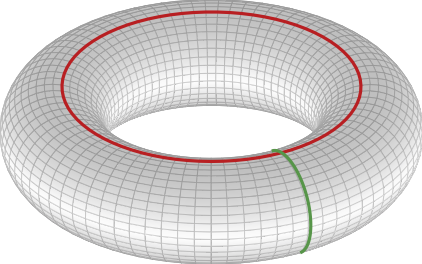
\includegraphics[width=0.4\textwidth]{./figures/LSR/torus.png}
    \caption{For a torus, the first Betti number is $b_1 = 2$ , which can be intuitively understood as the number of circular holes.}
    \label{fig:betti_torus}
\end{figure}
%\medskip

%\end{document}
